% Compile by directly running 
%   pdflatex Slurm_Intro.tex 
%
%
%
%
%
\documentclass{beamer}
\usetheme{Copenhagen}
\usepackage[utf8]{inputenc}


%\usepackage{graphicx}
%\usepackage{subfigure}
%\usepackage{multimedia}
\usepackage{times}  % fonts are up to you
\usepackage{graphics}
\usepackage{amsmath}
\usepackage{media9}
\usepackage{hyperref}
\usepackage{psfrag}
\usepackage{pdfpages}
\usepackage{listings}
% enumitem is incompatible with beame
%\usepackage{enumitem}   % for letters based enumeration - https://tex.stackexchange.com/a/129960/84495
%\usepackage[style=authoryear]{biblatex}
%\bibliography{/Users/ali/Library/texmf/bibtex/bib/references}


\setbeamertemplate{bibliography item}[text]
%\usepackage[backend=bibtex, style=authoryear]{biblatex}
%\addbibresource{/Users/ali/Library/texmf/bibtex/bib/references.bib}
\newcommand{\customcite}[1]{\citeauthor{#1}, \citeyear{#1}}
\newcommand\smallFont{\fontsize{8}{7.2}\selectfont}   %Change font size.
\newcommand\mCite[1]{[\cite{#1}, \citetitle{#1}]}  %Prints name and title
\newcommand\FrameText[1]{
\begin{textblock*}{\paperwidth}(0pt,\textheight)
	\vspace{1.0cm}
    \raggedleft \smallFont #1
\end{textblock*}}

%Get rid of ugly copenhagen default symbol for enumerate
\setbeamertemplate{enumerate items}[default]   


% Create code text
% https://tex.stackexchange.com/questions/65291/code-snippet-in-text
\definecolor{codegray}{gray}{0.9}
\newcommand{\code}[1]{\colorbox{codegray}{\texttt{#1}}}



%Information to be included in the title page:
\title{Session 04 - Speeding things up with parallel processing}
\author{Ali Snedden}
\institute{Nationwide Children's Hospital}
\date{May 02, 2023}
 
 
\begin{document}
 
\frame{\titlepage}

\begin{frame}
\frametitle{How to Connect}
Windows:
\begin{itemize}
    \item Open PuTTY
    \item Window Session $\Rightarrow$ Host Name field : \code{username@r1pl-hpcf-log01}
    \item Click ``Open" to log in.
    \item Enter password
\end{itemize}

Mac:
\begin{itemize}
    \item Open Terminal (Finder $\Rightarrow$ Utilities $\Rightarrow$ Terminal)
    \item \code{ssh -X username@r1pl-hpcf-log01}
\end{itemize}
\end{frame}



\begin{frame}
\frametitle{What is a computer?}
\begin{picture}(320,250)  %must be related to where it is centered
\put(-25, 100){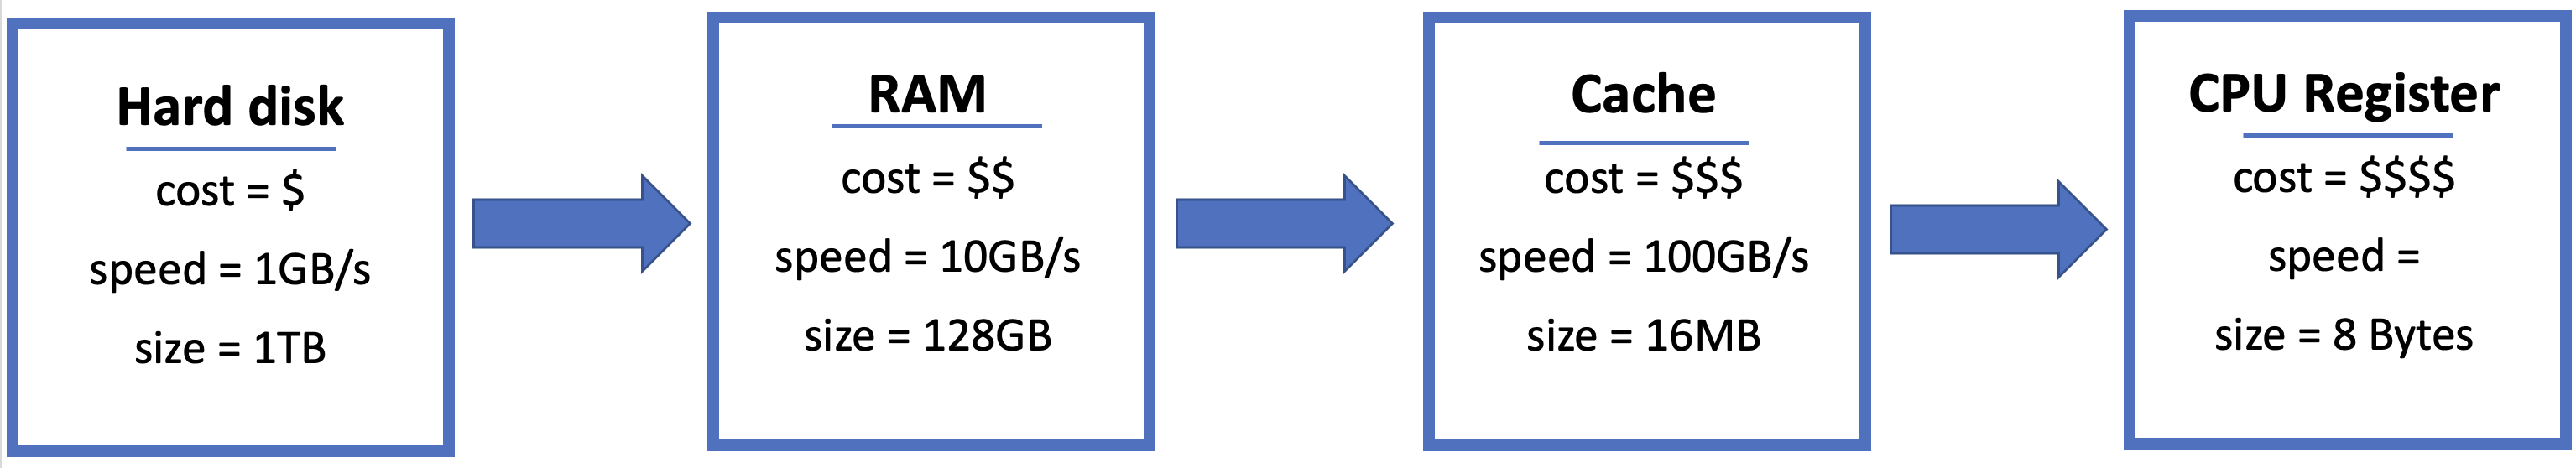
\includegraphics[height=0.90in]{images/what_is_a_computer.png}}
\end{picture}
\end{frame}


% Make 2 column, add icons to the right
\begin{frame}
\frametitle{What do you use your computer for?}
\begin{itemize}
    \item Composing and checking email.
    \bigskip
    \pause
    \item Using a web browser.
    \bigskip
    \pause
    \item Writing documents (e.g. papers, grants)
    \bigskip
    \pause
    \item Doing analysis.
\end{itemize}
\end{frame}


\begin{frame}
\frametitle{What do you use your computer for?}
Have you ever had an analysis that was too big or bogged down your computer?
%\pause
%\bigskip
%Enter : supercomputing
\end{frame}


\begin{frame}
\frametitle{Why use a supercomputer?}
\begin{itemize}
    \item Data set too large
    \bigskip
    \pause
    \item Analysis takes too much time
    \bigskip
    \pause
    \item Combination of the two
\end{itemize}
\end{frame}


\begin{frame}
\frametitle{Why use a supercomputer?}
Advantages :
\begin{itemize}
    \pause
    \item Offload analysis to a server so you can use your laptop again
    \medskip
    \pause
    \item Can do many tasks at once, less wall time
    \medskip
    \pause
    \item Have access to beefy machines that can handle large datasets
    \medskip
    \pause
    \item Expert support, e.g. software installation, advice, programming expertise.
    \medskip
    \pause
    \item Free in cost at NCH.
    \pause
\end{itemize}
\bigskip
Disadvantages :
\begin{itemize}
    \pause
    \item Learning curve (e.g. Linux, Slurm)
\end{itemize}
\end{frame}


\begin{frame}
\frametitle{How do you use a supercomputer?}
Use parallelization 
\pause
\begin{itemize}
    \item Take your task and break it up into many components that can be run concurrently.
\bigskip
\end{itemize}
\pause

Examples :
\pause
\begin{itemize}
    \item You have many sequencing files, they can all be aligned independently.
    \medskip
    \pause
    \item Matrix multiplication and other linear algebra operations   %% ADD IMAGE HERE
    \medskip
    \pause
    \item Large $N$-body or hydrodynamic simulations (e.g. weather models)      %% ADD IMAGE HERE
\end{itemize}
\end{frame}


\begin{frame}
\frametitle{Serial Computing Example}
\begin{picture}(320,250)  %must be related to where it is centered
\put(-25, 70){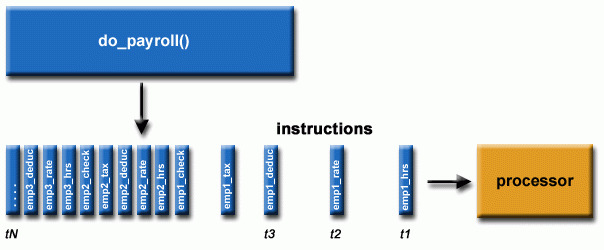
\includegraphics[height=2.00in]{images/serial_payroll.jpg}}
\end{picture}
\end{frame}


\begin{frame}
\frametitle{Parallel Computing Example}
\begin{picture}(320,250)  %must be related to where it is centered
\put(15, 70){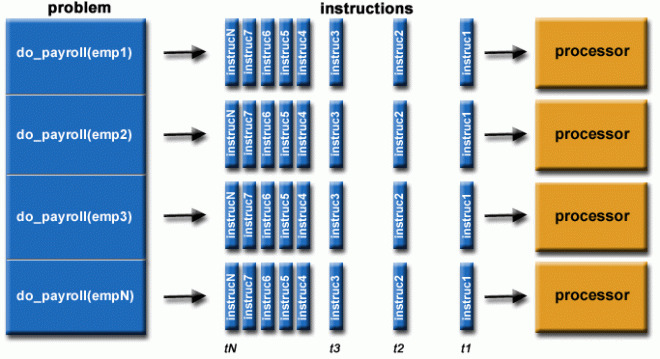
\includegraphics[height=2.0in]{images/parallel_payroll.jpg}}
\end{picture}
\end{frame}


\begin{frame}
\frametitle{Parallelization Concepts}
\begin{picture}(320,250) 
\visible<2-7>{\put(200, 145){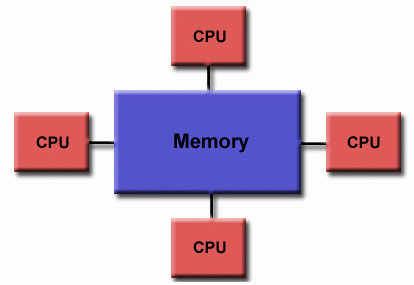
\includegraphics[height=1.25in]{images/shared_mem.jpg}}}
\visible<5-7>{\put(165, 50){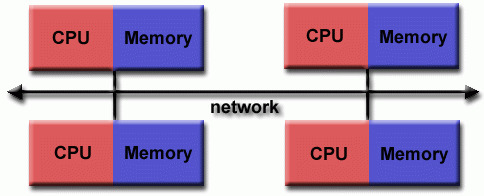
\includegraphics[height=0.95in]{images/distributed_mem.jpg}}}
\put(-20, 245){\begin{minipage}[t]{0.6 \linewidth}
{
%Parallelization:
\begin{itemize}
    \item Shared memory
        \pause
        \begin{enumerate}
            \item All memory used is within the same physical computer
            \pause
            \item Often used for 'embarrassingly parallizeable' problems
            \pause 
            \item Protocals 
                \begin{itemize}
                    \item C/C++/Fortran : OpenMP
                    \item R : parapply package
                    %\item Python : multiprocessing module
                \end{itemize}
        \end{enumerate}
    \pause
    \bigskip
    \item Distributed memory
        \begin{enumerate}
            \item Memory is distributed amongst multiple computers
            \pause
            \item Protocals 
                \begin{itemize}
                    \item C/C++/Fortran : MPI
                    \item Any language : Server-Client model over ports
                \end{itemize}
            \pause
            \item \textbf{\small UNCOMMON IN BIOINFORMATICS}
        \end{enumerate}
\end{itemize}
}
\end{minipage}}
\end{picture}
\end{frame}
 

\begin{frame}
\frametitle{How to use parallelization}
Many tools already have parallelization built in, e.g.
\begin{itemize}
    \item \code{hisat2 -p 12 -x index ... }
    \bigskip
    \pause
    \item \code{parapply}
    \bigskip
    \pause
    \item \code{numpy} with LAPACK
    \bigskip
    \pause
    \item Slurm
\end{itemize}
\end{frame}


\begin{frame}
\frametitle{Increasing Benefits of Parallelization}
\begin{picture}(320,250)  %must be related to where it is centered
\put(-30, -50){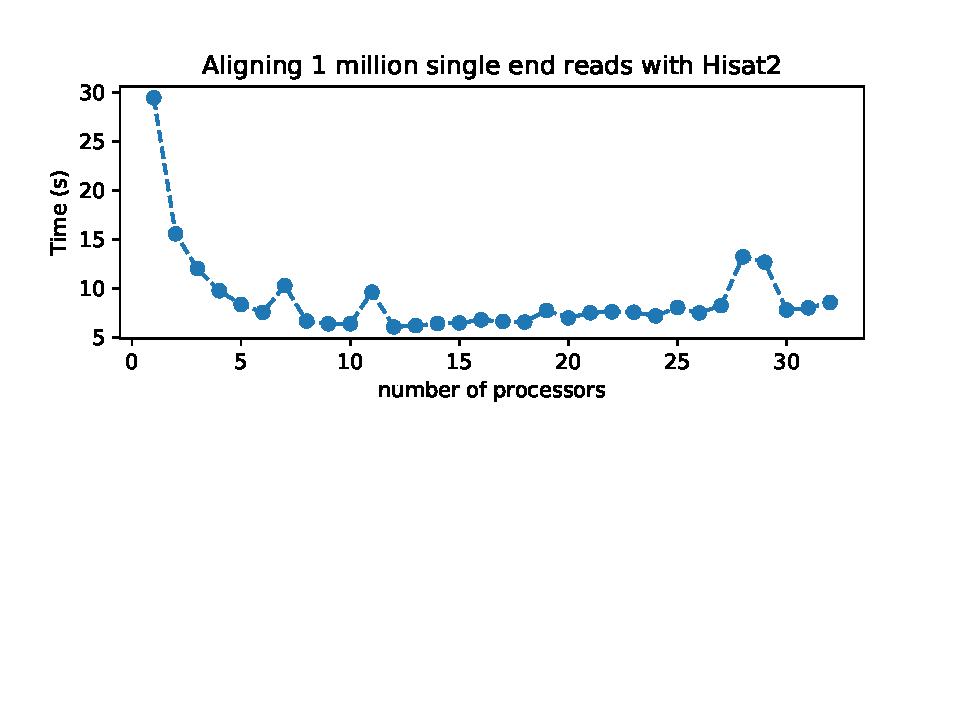
\includegraphics[height=3.75in]{images/hisat2_align_1m_reads.pdf}}
\end{picture}
\end{frame}

%\begin{frame}
%\frametitle{What is Slurm?}
%Need method for managing cluster resources.
%\bigskip
%\begin{itemize}
%    \pause
%    \item Enter SLURM - A Workload Manager
%    \bigskip
%    \pause
%    \begin{enumerate}
%        \item Permits efficient (and fair) utilization of Cluster resources.
%        \pause
%        \bigskip
%        \item This is your interface with the computer cluster
%    \end{enumerate}
%\end{itemize}
%\end{frame}
%

\begin{frame}
\frametitle{What is Slurm?}
\begin{picture}(320,250)  %must be related to where it is centered
\put(40, 18){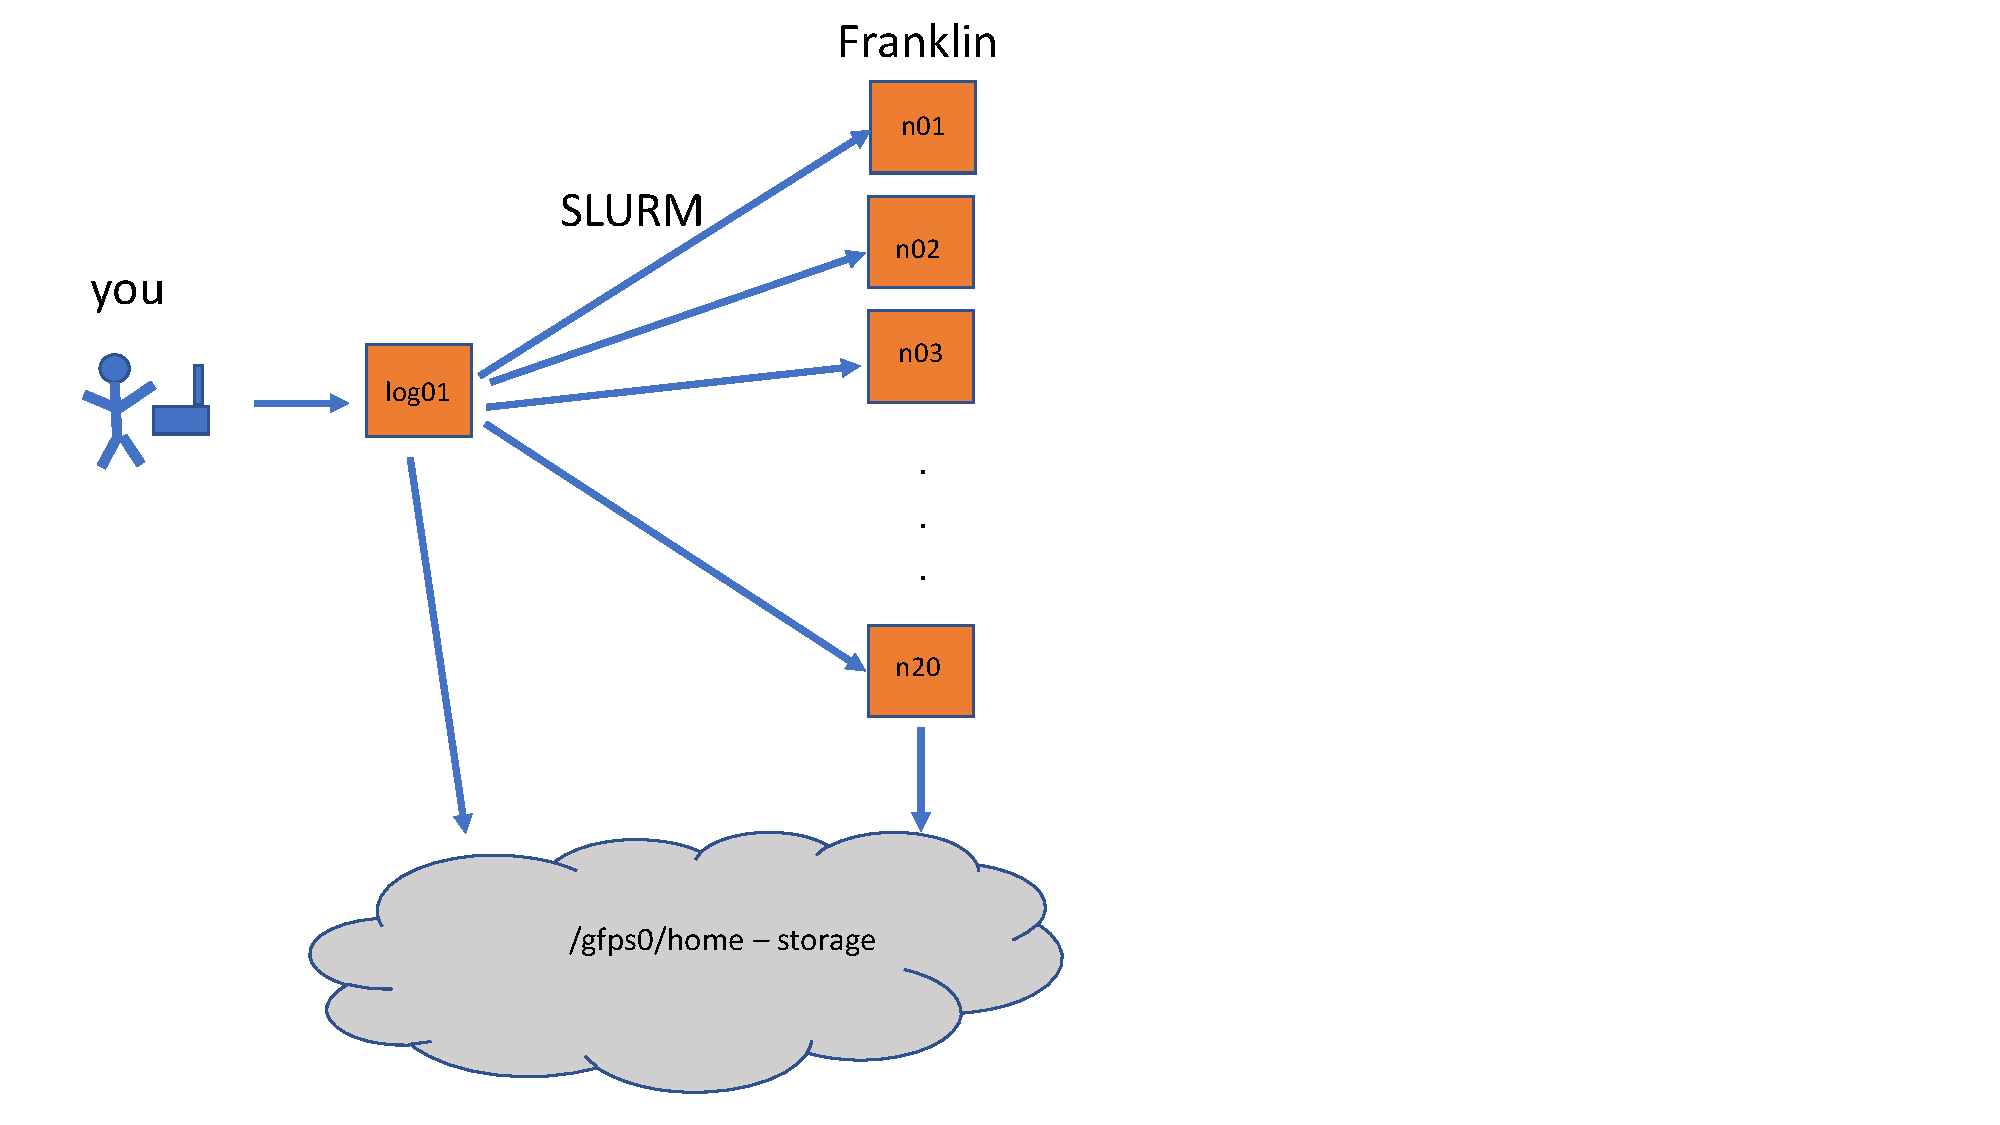
\includegraphics[height=3.25in]{images/franklin-cluster.pdf}}
\end{picture}
\end{frame}



%\begin{frame}
%\frametitle{Slurm Concepts}
%\begin{itemize}
%    \item Job
%    \pause 
%    \begin{enumerate}
%        \item Primary way of requesting resources
%        \pause
%        \item Composed of one or more Steps
%    \end{enumerate}
%    \bigskip
%    \pause
%    \item Step
%    \begin{enumerate}
%        \item A way of dividing the resources allocated
%        \pause
%        \item Can be run serially or in parallel within a job
%        \pause
%        \item Composed of one or more Tasks
%    \end{enumerate}
%    \bigskip
%    \pause
%    \item Task
%    \begin{enumerate}
%        \item Composed of one or more CPUs
%    \end{enumerate}
%    \bigskip
%\end{itemize}
%\end{frame}


%\begin{frame}
%\frametitle{Franklin}
%A typical job on Franklin : 
%\bigskip
%\begin{itemize}
%    \item 1 Node 
%    \bigskip
%    \pause
%    \item 1 Task
%    \bigskip
%    \pause
%    \item Multiple CPUs
%    \bigskip
%    \pause
%\end{itemize}
%Complicated jobs may benefit from utilizing multiple steps and tasks, most jobs will not.
%\end{frame}


%\begin{frame}
%\frametitle{How to use Slurm?}
%\begin{itemize}
%    \item \code{sbatch} - Non-interactive bash script
%    \bigskip
%    \pause
%    \item \code{srun} - Interactive sessions 
%    \bigskip
%\end{itemize}
%\end{frame}


%\begin{frame}
%\frametitle{sbatch}
%Examples of Usage:
%\bigskip
%\begin{itemize}
%    \item \code{sbatch myscript.sh}
%    \bigskip
%    \pause
%    \item \code{sbatch --cpus-per-task=20 myscript.sh}
%    \bigskip
%    \pause
%    \begin{enumerate}
%        \item NOTE : specifying 20 cores, will NOT magically make your script use 20 cores.
%                     You will need to specify that within your shell script \code{myscript.sh}
%    \end{enumerate}
%    \pause
%    \item \code{sbatch --gres=gpu myscript.sh}
%    \bigskip
%\end{itemize}
%\end{frame}



%\begin{frame}
%\frametitle{sbatch}
%Two ways to pass arguments to sbatch
%\smallskip
%\begin{itemize}
%    \item Command line
%        \smallskip
%        \begin{enumerate}
%            \item E.g. \code{sbatch OPTIONS myscript.sh}
%            \pause
%            \smallskip
%            \item Popular \code{OPTIONS}
%            \begin{enumerate}[a)]
%                \item \code{--cpus-per-task=} 
%                \pause
%                \smallskip
%                \item \code{--partition=himem}
%                \pause
%                \smallskip
%                \item \code{--gres=gpu}
%            \end{enumerate}
%            \pause
%            \smallskip
%            \item Preempts options set in bash script
%        \end{enumerate}
%        \smallskip
%
%    \pause
%    \item In Bash Script, \code{myscript.sh}
%        \smallskip
%        \begin{enumerate}
%            \item Popular \code{OPTIONS}
%            \begin{enumerate}[a)]
%                \item \code{\#SBATCH --cpus-per-task=} 
%                \pause
%                \smallskip
%                \item \code{\#SBATCH --partition=himem}
%                \pause
%                \smallskip
%                \item \code{\#SBATCH --gres=gpu}
%            \end{enumerate}
%        \end{enumerate}
%\end{itemize}
%\end{frame}




\begin{frame}[fragile]
\frametitle{sbatch}
Example \code{myscript.sh}: 
\begin{lstlisting}[backgroundcolor = \color{codegray}, language = Bash, showstringspaces=false]
    #!/bin/bash
    #SBATCH --cpus-per-task=10
    set -e
    echo "Hello World"
    sleep 30
\end{lstlisting}
\bigskip
\bigskip
Submit with \code{sbatch myscript.sh}
\end{frame}


%\begin{frame}[fragile]
%\frametitle{sbatch}
%Output from batch script (\code{slurm-1795906.out}), will have some of the below information (some columns abbreviated for clarity)
%\begingroup
%\tiny
%\begin{lstlisting}[backgroundcolor = \color{codegray}, language = Bash, showstringspaces=false]
%Hello World
%Job Statistics for 179:
%       JobID   User Start End   Elapsed  MaxRSS   TotalCPU State Exit  NodeList ReqTRES
%------------ ------ ----- --- --------- ------- ---------- ----- ---- --------- ----------------
%         179 user01 ..... ...  00:00:00          00:00.009 COMPL  0:0    node01  cpu=1,mem=6144M
%   179.batch        ..... ...  00:00:00       0  00:00.008 COMPL  0:0    node01
%  179.extern        ..... ...  00:00:00       0   00:00:00 COMPL  0:0    node01
%CPU Efficiency: 0.00% of 00:00:00 core-walltime
%\end{lstlisting}
%\endgroup
%\end{frame}


%\begin{frame}[fragile]
%\frametitle{sbatch}
%Himem partition allocation example \code{myscript\_himem.sh}: 
%\begin{lstlisting}[backgroundcolor = \color{codegray}, language = Bash, showstringspaces=false]
%    #!/bin/bash
%    #SBATCH --cpus-per-task=2
%    #SBATCH --partition=himem
%    set -e
%    echo "Hello World"
%    sleep 30
%\end{lstlisting}
%\bigskip
%\bigskip
%Submit with \code{sbatch myscript\_himem.sh}
%\end{frame}


%\begin{frame}[fragile]
%\frametitle{sbatch}
%GPU allocation example \code{myscript\_gpu.sh}: 
%\begin{lstlisting}[backgroundcolor = \color{codegray}, language = Bash, showstringspaces=false]
%    #!/bin/bash
%    #SBATCH --cpus-per-task=2
%    #SBATCH --gres=gpu
%    set -e
%    echo "Hello World"
%    sleep 30
%\end{lstlisting}
%\bigskip
%\bigskip
%Submit with \code{sbatch myscript\_gpu.sh}
%\end{frame}



\begin{frame}[fragile]
\frametitle{sbatch}
Broken Example \code{myscript\_broken.sh}: 
\begin{lstlisting}[backgroundcolor = \color{codegray}, language = Bash,showstringspaces=false]
    #!/bin/bash
    #SBATCH --cpus-per-task=2
    #SBATCH --partition=himem
    #SBATCH --mail-user=First.Last@gmail.com
    #SBATCH --mail-type=FAIL,TIME_LIMIT_90
    set -e
    echo "I'm looking in the forbidden location"
    ls /root/
    echo "I never make it here"
\end{lstlisting}
\bigskip
\bigskip
Submit with \code{sbatch myscript\_broken.sh}
\end{frame}



%\begin{frame}
%\frametitle{srun}
%\code{srun} - Interactive allocation 
%\bigskip
%\begin{itemize}
%    \item Use when needing to interactively run long processes. E.g.
%        \begin{enumerate}
%            \item compiling
%            \pause 
%            \item developing and testing workflows
%            \pause 
%            \item downloading data
%            \pause 
%            \item GUI editors, e.g. RStudio
%            \pause 
%            \item Plotting, e.g. gnuplot, matplotlib
%            \pause 
%        \end{enumerate}
%    \pause
%    \item Example command : \code{srun --x11 --cpus-per-task=2 --pty bash}
%        \pause
%        \begin{enumerate}
%            \item \code{--x11} option only needed for GUIs (e.g. RStudio)
%            \pause
%            \item For \code{--x11} to work, you must have X11 server installed
%            \pause
%            \begin{enumerate}[a)]
%                \item Vcxsrv for Windows
%                \pause
%                \item XQuartz for Mac
%            \end{enumerate}
%        \end{enumerate}
%    \pause
%    \item \code{srun} takes all same command line options as \code{sbatch}
%\end{itemize}
%\end{frame}


\begin{frame}
\frametitle{Monitoring Jobs Progress}
There are several ways to monitor jobs progress.  
\bigskip
\begin{itemize}
    \item \code{squeue}
    \pause
    \bigskip
    \item \code{scontrol}
\end{itemize}
\end{frame}


\begin{frame}[fragile]
\frametitle{Monitoring Jobs Progress}
\code{squeue}, e.g. 
\begingroup
\tiny
\begin{lstlisting}[backgroundcolor = \color{codegray},showstringspaces=false]
   JOBID PARTITION          NAME     USER ST       TIME  NODES      CPUS NODELIST(REASON)
 1791312   general gromacs_test_   user01  R 9-21:30:30      1        20 node02
 1791313   general gromacs_test_   user01  R 9-21:30:09      1        20 node03
 1791316   general          his1   user01  R 9-21:28:56      1        20 node06
 1791317   general          his1   user01  R 9-21:28:53      1        20 node07
 1794106   general          test   user02  R 3-20:17:31      1        20 gpu03
 1794236   general          bash   user03  R 2-23:33:53      1         1 node01
\end{lstlisting}
\endgroup
\end{frame}



\begin{frame}[fragile]
\frametitle{Monitoring Jobs Progress}
\code{scontrol}, e.g. \code{ scontrol show jobid 1794106}
\begingroup
\tiny
\begin{lstlisting}[backgroundcolor = \color{codegray},showstringspaces=false]
JobId=1794106 JobName=test
   UserId=user02(600) GroupId=group01(1181939003) MCS_label=N/A
   Priority=28575 Nice=0 Account=gdpairlab QOS=normal
   JobState=RUNNING Reason=None Dependency=(null)
   Requeue=1 Restarts=0 BatchFlag=1 Reboot=0 ExitCode=0:0
   RunTime=3-20:25:41 TimeLimit=7-00:00:00 TimeMin=N/A
   SubmitTime=2019-04-15T12:30:01 EligibleTime=2019-04-15T12:30:01
   StartTime=2019-04-15T12:30:02 EndTime=2019-04-22T12:30:02 Deadline=N/A
   PreemptTime=None SuspendTime=None SecsPreSuspend=0
   LastSchedEval=2019-04-15T12:30:02
   Partition=general AllocNode:Sid=qmaster01:20116
   ReqNodeList=gpu03 ExcNodeList=(null)
   NodeList=gpu03
   BatchHost=gpu03
   NumNodes=1 NumCPUs=20 NumTasks=1 CPUs/Task=20 ReqB:S:C:T=0:0:*:*
   TRES=cpu=20,mem=120G,node=1,billing=20,gres/gpu=1
   Socks/Node=* NtasksPerN:B:S:C=0:0:*:* CoreSpec=*
   MinCPUsNode=20 MinMemoryCPU=6G MinTmpDiskNode=0
   Features=(null) DelayBoot=00:00:00
   Gres=gpu:1 Reservation=(null)
   OverSubscribe=OK Contiguous=0 Licenses=(null) Network=(null)
   Command=/gpfs0/home/group01/user02/ram_test/start_gtn.sh
   WorkDir=/gpfs0/home/group01/user02/ram_test
   StdErr=/gpfs0/home/group01/user02/ram_test/test_1794106.out
   StdIn=/dev/null
   StdOut=/gpfs0/home/group01/user02/ram_test/test_1794106.out
   Power=
\end{lstlisting}
\endgroup
\end{frame}


%\begin{frame}[fragile]
%\frametitle{Homework 1 - Illustrating jobs, steps and tasks}
%\end{frame}




%\begin{frame}[fragile]
%\frametitle{Homework 1 - Illustrating jobs, steps and tasks}
%Consider the following scripts
%
%\medskip
%\code{step.sh}
%\begingroup
%\small
%\begin{lstlisting}[backgroundcolor = \color{codegray},showstringspaces=false, language=Bash]
%#!/bin/bash
%#SBATCH --cpus-per-task=10
%#SBATCH --tasks-per-node=2
%srun --ntasks=1 bash other.sh first_step &
%srun --ntasks=1 bash other.sh second_step &
%wait
%\end{lstlisting}
%\endgroup
%
%
%\medskip
%\code{other.sh}
%\begingroup
%\small
%\begin{lstlisting}[backgroundcolor = \color{codegray},showstringspaces=false, language=Bash]
%#!/bin/bash
%date
%echo "Hello from $1"
%sleep 30
%echo "World from $1"
%date
%\end{lstlisting}
%\endgroup
%\end{frame}
%
%
%
%\begin{frame}
%\frametitle{Homework 1 - Illustrating jobs, steps and tasks}
%\begin{itemize}
%    \item Submit job \code{step.sh}
%    \bigskip
%    \item Remove the \code{\&} at the end of the lines. What happens?
%    \bigskip
%    \item Remove the \code{\&} at the end of the lines along with \code{wait}. What happens?
%    \bigskip
%    \item Remove the \code{--ntasks=1}, along with \code{\&} and \code{wait}. What happens?
%    \bigskip
%    \item Try different combinations.
%\end{itemize}
%\end{frame}


\begin{frame}
\frametitle{Resources}
\begin{itemize}
    \item \href{https://hpc.llnl.gov/documentation/tutorials/introduction-parallel-computing-tutorial}{\color{blue}Introduction to Parallel Computing Tutorial - LLNL}
    \item \href{https://stackoverflow.com/a/46532581/4021436}{\color{blue}How Slurm Tasks, jobs and steps relate - Stackoverflow}
    \bigskip
\end{itemize}
\end{frame}

\begin{frame}
\frametitle{EXTRA SLIDES}
\large EXTRA SLIDES
\end{frame}

\begin{frame}
\frametitle{Cluster Architecture}
Type of hardware available
\begin{itemize}
    \item High Memory (himem)
    \begin{enumerate}
        \item 2.0 TB RAM
        \item 48 cores 
        \item AMD EPYC 7402 CPU
    \end{enumerate}
    \bigskip
    \pause
    \item General Purpose (default)
    \begin{enumerate}
        \item 256 GB RAM
        \item 32 cores 
        \item AMD EPYC 7302 CPU
    \end{enumerate}
    \bigskip
    \pause
    \item GPU 
    \begin{enumerate}
        \item 256GB RAM 
        \item 32 cores 
        \item AMD EPYC 7302 CPU
        \item NVidia A100 and V100 GPUs available
    \end{enumerate}
\end{itemize}
\end{frame}


\begin{frame}
\frametitle{Cluster Architecture}
Storage 
\begin{itemize}
    \item 664 TB of storage available
    \pause
    \item Flexible limits on user storage - be responsible.
          It takes everyone's cooperation to have this nice feature.
    \pause
    \item Not intended for archival or long term storage.
        \begin{enumerate}
              \item Be sure to back up your important data and code elsewhere
              \pause
              \item If data center goes up in smoke, your research, time and grant money may as well.
        \end{enumerate}
    \pause
    \item PHI permitted
\end{itemize}
\pause
Networking:
\begin{itemize}
    \item 100 Gb/s Infiniband fabric available
\end{itemize}
\end{frame}


\end{document}
